\section{METODOLOGI}
\label{chap:desainimplementasi}

% Ubah bagian-bagian berikut dengan isi dari desain dan implementasi

% Penelitian ini dilaksanakan sesuai \lipsum[1][1-5]

\subsection{Data dan Peralatan / Data dan Alat Bantu / Material}
\label{sec:perlengkapan}


\begin{enumerate}
  \item Dataset
  \par Untuk mencapai hasil training model, akan digunakan dataset Safety Helmet Detection yang merupakan dataset berisi 5000 gambar personil proyek yang menggunakan helm proyek dan yang tidak. Pada dataset ini sudah diberikan label pada annotation untuk tiap gambarnya. \cite{larxel_2020}
  \par Larxel, “Safety helmet detection,” Kaggle, 11-Aug-2020. [Online]. 
  Available: https://www.kaggle.com/andrewmvd/hard-hat-detection. [Accessed: 20-Oct-2021].

  \item Alat Bantu
  \begin{enumerate}
    \item Anaconda
    \par Anaconda sendiri merupakan package distribution yang dibuat khusus untuk data science. Anaconda biasanya digunakan untuk membuat environment baru untuk mengisolasi proyek dan menginstall package untuk keperluan tertentu. Pada penelitian ini akan digunakan untuk membantu penulis dalam mengumpulkan package - package yang diperlukan untuk melakukan proses training dan pengembangan sistem.\cite{pankajmathur_2018}

    \item Python 3.7
    \par Python sendiri adalah bahasa pemrograman high level yang sudah terinterpretasi dan berbasis objek. Struktur data yang sudah ada di dalam python dan penulisan syntax yang sederhana dan mudah dipahami dapat meningkatkan performa pengerjaan. Pada penelitian ini python digunakan karena merupakan bahasa pemrograman yang cocok untuk data science mengingat struktur data di python yang dinamis. Selain itu python juga sudah termasuk saat menginstall Anaconda \cite{python.org}

    \item Visual Studio Code
    \par Visual Studio Code adalah source code editor yang ramah performa dan mudah digunakan untuk segala bentuk keperluan penulisan text sehari - harinya. Visual Code mendukung banyak bahasa pemrograman dan menyediakan fitur addons yang digunakan untuk mendownload package untuk berbagai macam kebutuhan berbeda. Pada penelitian ini Visual Studio Code digunakan untuk menulisa script python yang akan digunakan untuk training, pengembangan sistem, dan keperluan lainyna yang sekiranya dibutuhkan pada penelitian ini dan dapat diselesaikan dengan visual studio code.\cite{microsoft_2021}

  \end{enumerate}


\end{enumerate}



\subsection{Metodologi Penelitian}
\label{metodologipenelitian}

\begin{figure}[ht]
  \centering
  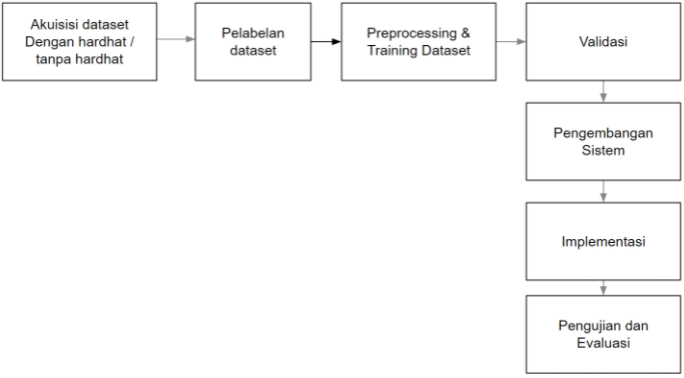
\includegraphics[scale=0.4]{gambar/blockdiagram-helmetdetection.png}
  \caption{Block Diagram Penelitian Deteksi Helm Keselamatan kerja Menggunakan CNN}
  \label{fig:blockdiagramhelmetdetection}  
\end{figure}

\begin{enumerate}
  \item Akuisisi Dataset
  \par Dataset yang diperlukan untuk melakukan training yaitu dataset gambar personil proyek yang menggunakan helm keselamatan kerja dan yang tidak. Seperti disebutkan sebelumnya sudah didapatkan dataset Safety Helmet Dataset yang berisi 5000 gambar personil proyek yang menggunakan helm dan yang tidak.
  
  \item Pelabelan dataset
  \par Dataset yang didapatkan dari kaggle sebenarnya sudah memiliki anotasi untuk tiap gambarnya, tetapi dengan kebutuhan tambahan untuk bounding box kepala hingga dada maka diperlukan anotasi tambahan.
  
  \item Preprocessing Dataset dengan Roboflow
  \par Sebelum dapat digunakan untuk training menggunakan YOLOv5, dataset yang ditapatkan perlu di\emph{pre-process}. Untuk saat ini pre-process baru meliputi pengubahan ukuran gambar dan konversi format anotasi ke format \emph{.xml} unyuk YOLOv5

  \item Training Dataset dan Validasi

  \item Pengembangan Sistem
  \par Perlu dilakukannya pengembangan sistem yang dapat menerima input video real time dari kamera yang lalu dapat melakukan identifikasi penggunaan helm dan tidak yang dimana dilakukan dengan menggunakan model yang sudah dibuat. 

  \item Implementasi
  \par Sistem yang sudah akan dikerahkan pada pengaplikasian dunia nyata seperti pada proyek konstruksi

  \item Pengujian dan Evaluasi
  \par Dari proses implementasi akan dilakukan pengujian keberhasilan dan keefektifan sistem saat dikerahkan pada implementasi dunia nyata.

\end{enumerate}


% % Contoh pembuatan potongan kode
% \begin{lstlisting}[
%   language=C++,
%   caption={Program halo dunia.},
%   label={lst:halodunia}
% ]
% #include <iostream>

% int main() {
%     std::cout << "Halo Dunia!";
%     return 0;
% }
% \end{lstlisting}

% \lipsum[2-3]

% % Contoh input potongan kode dari file
% \lstinputlisting[
%   language=Python,
%   caption={Program perhitungan bilangan prima.},
%   label={lst:bilanganprima}
% ]{program/bilangan-prima.py}

% \lipsum[4]
